\newpage % Rozdziały zaczynamy od nowej strony.
\section{Przegląd istniejących rozwiązań klasyfikacji informacji}
W poniższym rozdziale przedstawione zostaną wybrane metody służące do klasyfikacji informacji pod względem zawierania przez nich prawdy lub fałszu. Istnieją dwa główne typy mechanizmów: manualny - wymagający pracy człowieka oraz automatyczny gdzie do klasyfikacji używane są różne typy algorytmów. Automatyczne dodatkowo można wyraźnie rozróżnić pod kątem danych jakie są używane w\,celu klasyfikowania treści. 
\subsection{Rozwiązania manualne}
Do tej grupy zostały zakwalifikowane rozwiązania które w\,dużej mierze lub całkowicie polegają na pracy człowieka. Praca ta polega na manualnej decyzji osoby czy przedstawiony jej tekst zawiera prawdę czy jest dezinformujący. Sposoby tej pracy różnią się zaangażowaniem oceniającej osoby. Jako eksperta traktujemy osobę która poświęca czas i\,posiadaną wiedzę aby poprzeć swoją opinię dowodami z\,wiarygodnych źródeł. Innym sposobem jest użycie tzw. crowdsourcingu który polega na zbieraniu opinii dużej liczby użytkowników, którzy niekoniecznie są całkowicie wiarygodni. 
\subsubsection{Praca ekspertów}
Badanie rzetelności faktów zawartych w\,artykułach lub w\,wypowiedziach osób publicznych jest często zadaniem skomplikowanym oraz czasochłonnym. Są jednak inicjatywy poświęcone wykrywaniu fałszu lub niepełnej prawdziwości w\,publikowanych informacjach. Jednymi z\,najbardziej popularnych stron zajmujących się taką weryfikacją są Politifact\footnote{\url{https://www.politifact.com}} oraz Snopes\footnote{\url{https://www.snopes.com}} . Podejmują one głównie tematy związane ze polityką Stanów Zjednoczonych. Ich działanie polega na zatrudnianiu niezależnych dziennikarzy, których zadaniem jest wyszukiwanie źródeł weryfikujących wiarygodność informacji podawanych w\,sieci. Oceniają oni daną informację według ustalonej klasyfikacji. Aby być samemu być wiarygodnym zawsze podają źródła zarówno sprawdzanej informacji jak i\,materiałów użytych do wydania oceny. Dzięki temu użytkownik sam może zweryfikować swoją opinię. 
\par To rozwiązanie mimo oczywistych plusów, jakimi jest rzetelność i\,przejrzystość weryfikacji wierzytelności ma też znaczące minusy. Wymaga ono dużych nakładów pracy wykonanej przez specjalnie zatrudnionych w\,tym celu ekspertów. Metoda ta jest również czasochłonna zwłaszcza przy niejasnych przypadkach. Zwiększa to ryzyko, że kłamliwa informacja zostanie rozpowszechniona wśród większej liczby osób zanim zostanie zweryfikowana. Ponadto działanie takiego rozwiązania opiera się na założeniu, że użytkownicy czytają jedną z\,weryfikujących stron, co wymaga większego zaangażowania i\,może powodować pewną niedogodność dla standardowego odbiorcy. 
\subsubsection{Crowdsourcing}
Inną stosowaną metodą na wykrywanie fałszu jest crowdsourcing. Istnieją rozwiązania, które zbierają opinie użytkowników na temat prawdziwości lub nieszczerości konkretnych wypowiedzi umieszczanych w\,Internecie. Dzięki temu mogą one ostrzegać innych użytkowników przed zbytnią ufnością do czytanego źródła. Takie podejście wykorzystuje na przykład projekt fakenewsdetector.org\footnote{\url{https://fakenewsdetector.org/en}}. Jest to projekt opensource, który stworzył wtyczkę internetową o tej samej nazwie. Połączył on opisaną wyżej metodę jako zbieranie danych do uczenia maszynowego. Dzięki temu uczy się klasyfikować informacje świeżo opublikowane, które nie zdążyły być jeszcze przeczytane przez żadnego użytkownika. 
\par Fiskkit\footnote{\url{https://fiskkit.com}} jest platformą, która daje większe możliwości dyskusji nad artykułem niż przeciętne medium z\,artykułami. Platforma nie zawiera własnych artykułów, ale pozwala użytkownikom na importowanie ich z\,dowolnego źródła i\,daje możliwość dyskusji bezpośrednio nad każdym osobnym zdaniem w\,danym tekście. Użytkownicy mogą więc wskazywać dokładne fragmenty które uważają za fałszywe lub zbyt uproszczone.
\par Dużym minusem wykorzystania corwdsourcingu w\,ocenianiu prawdziwości artykułów powinien być brak zaufania do mas użytkowników. Osoby udzielające swojej opinii mogą być skrajnie stronnicze tak samo jak są przy udostępnianiu niepewnych informacji na portalach społecznościowych.

\subsection{Rozwiązania automatyczne}
Poniżej przedstawię kilka wybranych rozwiązań informatycznych działających w\,kierunku wykrywania fałszu lub stronniczości w\,artykułach i\,mediach społecznościowych. 
Warto na początku zaznaczyć, że większość istniejących prac skupia się na treściach intencjonalnie fałszywych, odrzucając teorie spiskowe, plotki, ponieważ te z\,definicji są trudniejsze do określenia czy są całkowicie fałszywe czy zawierają prawdę. Z\,rozpoznawania powinno się też wyłączyć satyrę, ponieważ ta działa na innych prawach. Portale publikujące teksty satyryczne zazwyczaj bezpośrednio podają do wiadomości użytkownika, że zawierają treści humorystyczne i\,informacje w\,nich zawarte nie powinny być traktowane poważnie.

\subsubsection{Style-based}
Rozważania nad używaniem metod przetwarzania języka naturalnego wywodzi się z\,założenia, że artykuły, które szerzą intencjonalną dezinformację różnią się stylem od artykułów prawdziwych. Może się to ujawniać na przykład w\,bardziej emocjonalnym słownictwie, poruszanych tematach lub skrajnej stronniczości.
\par Częstym zabiegiem wykorzystywanym do szerzenia dezinformacji w\,artykułach jest wykorzystywanie chwytliwego tytułu. Taka metoda często ma za zadanie zwabić czytelnika na kliknięcie w\,artykuł (tzw. clickbait). Oprócz takiego zastosowania równie często zdarza się, że sam tytuł może wyrażać fałszywe stwierdzenie natomiast treść artykułu naprostowuje je w\,stronę prawdy, użytkownik jednak nie dowie się o omylności tytułu, jeśli nie zdecyduje się przeczytać całości. W\,2017 zorganizowany został konkurs FakeNewsChallange\footnote{\url{http://www.fakenewschallenge.org}}, którego pierwszym etapem było stworzenie rozwiązania wykrywającego w\,jaki sposób treść artykułu odnosi się do jego tytułu. Może on bowiem zgadzać się lub nie zgadzać z\,tytułem. Artykuł może też omawiać dany temat ale nie wyrażać własnej opinii, możliwe jest też że treść dotyczy innego tematu niż tytuł. Rozwiązanie, które zostało ocenione najlepiej zostało stworzone przez grupę o nazwie Solat in the Swen. Stworzyli oni model oparty na połączeniu drzew decyzyjnych oraz głębokich sieci neuronowych. 
\par
Także w\,Polsce powstało badanie mające na celu sprawdzenia możliwości wykorzystania wiedzy psycholingwistycznej w\,celu rozpoznawania zdań zawierających fałsz\cite{wawer2019fact}. W\,tym celu zebrano 400 stwierdzeń od 200 uczestników. Jednak aby wykonać to badanie zdania zebrane w\,języku polskim zostały przetłumaczone na język angielski używając Google Translate. Mimo to dla zdań o silnie spolaryzowanych tematach otrzymano lepsze wyniki niż w\,przypadku testowania poprzez factchecking z\,wykorzystaniem portalu Wikipedia. 

\subsubsection{Knowladge-based}
Aby automatycznie wykrywać, czy informacja jest prawdziwa czy też nie można zastosować dostępne ustrukturalizowane bazy wiedzy takie jak DBpedia , która pobiera dane z\,Wikipedii tworząc sieć semantyczną. Jej celem jest uporządkowanie wiedzy, jaka istnieje w\,Internecie w\,formie grafu wiedzy.  Takie podejście sprawdziło się przy sprawdzaniu krótkich twierdzeń na temat historii, geografii czy rozrywki\cite{ciampaglia2015computational}. Wykorzystano tam zależność między bliskością zagadnień w\,grafie wskazujących na prawdziwość zdania, w\,którym występują. Wizualizację takiej metody przedstawiono na rysunku \ref{fig:barackObama} gdzie bazując na informacjach z\,Wikipedii starano się ustalić czy zdanie "Barack Obama jest muzułmaninem". Po lewej znajduje się informacja o postaci pobrana bezpośrednio z\,Wikipedii a\,po prawej ścieżka jaką przeszedł algorytm aby połączyć ze sobą dwa pojęcia: Barack Obama oraz islam. Liczby w\,nawiasach oznaczają ilość połączeń jaki posiada dana strona. Im wyższa to liczba tym niższą daje wartość do obliczenia końcowej wartości prawdopodobieństwa prawdy w\,badanym zdaniu. 

\begin{figure}[!h]
	\centering 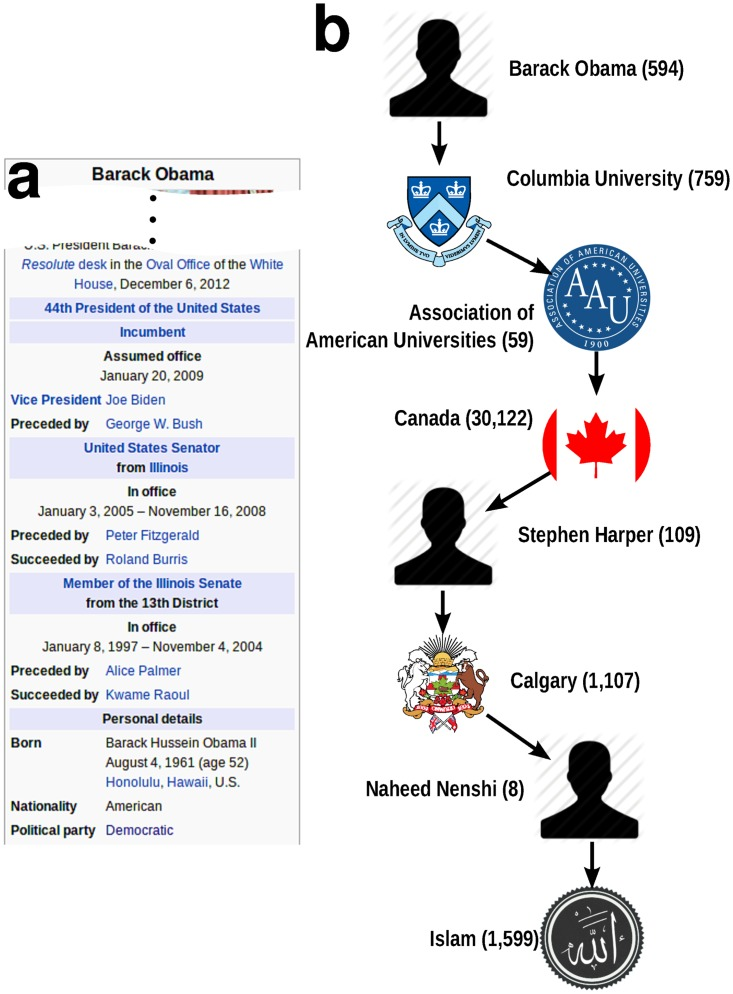
\includegraphics[width=0.5\linewidth]{img/barackObamaIsAMuslimNew.jpg}
	\caption{Wizualizacja zastosowania artykułów w\,Wikipedii do określenia prawdziwości stwierdzenia. źródło: \cite{ciampaglia2015computational}}
	\label{fig:barackObama}
\end{figure}
\par

\subsubsection{Context-based}
To podejście skupia się nie na treści prezentowanej informacji ale na jej kontekście. Jako kontekst można traktować autora tej informacji, serwis na którym się znajduje lub komentarze pozostawione przez odbiorców. Świetnym źródłem do zbierania tego typu informacji o kontekście są media społecznościowe. Ich idea polega na tym aby użytkownicy ingerowali w\,publikowane treści poprzez komentowanie, prowadzenie dyskusji i\,udostępnianie informacji większej grupie odbiorców.
\par
W obecnych czasach bardzo duże znaczenie mają media społecznościowe. Według badań z\,2018 roku 68\% ankietowanych pobiera wiedzę o aktualnych wydarzeniach właśnie z\,takich źródeł \cite{PewNewsUse2018}. Jest to wygodne i\,szybkie jednak bardzo podatne na manipulacje. Można jednak wykorzystać sieci zależności jakie tworzą źródła publikujące informacje z\,ich odbiorcami. Praca pod tytułem Some like it Hoax\cite{tacchini2017some} skupiła się na działalności użytkowników platformy Facebook jakim są ’polubienia’ postów. Projekt pobrał 15,500 postów polubionych przez ponad 900 tysięcy użytkowników. Aby wykrywać potencjalny fake news wykorzystał stworzony wcześniej podział stron na naukowe oraz o tematyce konspiracyjnej\cite{bessi2015science}. Wykorzystując fakt, że większość użytkowników ograniczała swoją aktywność tyko do postów należących do tylko jednej z\,tych kategorii, ale istnieje też niemała grupa akceptująca oba rodzaje stron możliwe było osiągnięcie bardzo wysokich wyników klasyfikacji postów do odpowiedniej kategorii. 
\par
Powstał również portal o nazwie Hoaxy\cite{shao2016hoaxy} na którym można prześledzić w\,formie grafu jak udostępniane są posty publikowane na Twitter. Dzięki tej aplikacji można zobaczyć, jak rozprzestrzenia się wskazany przez nas post, w\,czasie między kolejnymi użytkownikami. Przykład wykorzystania ukazano na rysunku \ref{fig:hoaxyTrump}. Znajduje się na nim wizualizacja sieci rozprzestrzeniania się wiadomości opublikowanej pierwotnie na koncie Donalda Trumpa dnia 03.05.2019. W\,czasie dwóch dni informacja ta została przekazana ponad 22 tysiące razy.
\begin{figure}[!h]
	
	\centering 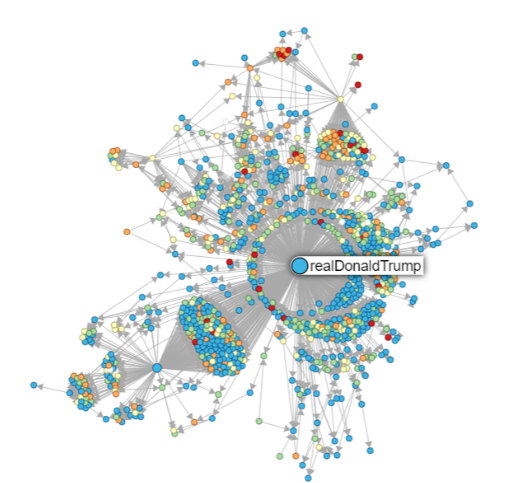
\includegraphics[width=0.5\linewidth]{img/hoaxy.png}
	\caption{Sieć rozprzestrzeniania się wiadomości na platformie Twitter na przykładzie wiadomości Donalda Trumpa. źródło: \url{https://hoaxy.iuni.iu.edu}}
	\label{fig:hoaxyTrump}
\end{figure}
\par
Innym podejściem do klasyfikacji źródeł publikujących informacje jest wykorzystanie odniesień jakie robią między sobą strony internetowe. Taką metodę wykorzystywał Pagerank działający dla Google. Wyznaczając rangę ważności strony brał on pod uwagę rangę stron, do których dana storna się odwoływała. Innym algorytmem wykorzystującą sieć skierowaną którą tworzą odniesienia jakie występują między stronami jest HITS. Opisuje on dwa typy stron: autorytety i\,koncentratory. Autorytetem jest strona, która jest często cytowana przez inne strony, natomiast koncentratorem jest strona, która wskazuje na wiele ważnych stron. Fakt, że strony internetowe zawierają odniesienia do innych stron można wykorzystać też do badania wiarygodności portali internetowych pod względem prawdziwości publikowanych informacji. Badania wykazały, że wykrywanie kłamliwych źródeł w\,takim grafie odbywa się z\,dużo większym sukcesem niż próba wykrycia tego przy zastosowaniu metod lingwistycznych bezpośrednio na publikowanych artykułach\cite{fairbanks2018credibility}. Wykorzystano w\,nich bazę danych pochodzącą z\,The Global Database o Events Language and Tone\footnote{\url{https://www.gdeltproject.org}}. Z\,pobranych artykułów podających linki zewnętrzne stworzono graf zawierający ponad 19 tysięcy unikalnych źródeł połączonych ponad 32 tysiącami linków. Oznaczenia wiarygodności dokonano na poziomie źródła, wykorzystano do tego istniejące oceny stron wykonane przez portal Media Bias Fact Check\footnote{\url{https://mediabiasfactcheck.com}}. Dzięki wykorzystaniu odpowiedniego algorytmu propagacji nie było wymagane, aby wszystkie źródła w\,grafie miały na wstępie zadeklarowaną ocenę. 